\section{Termes corrélés}
  Pour identifier les termes corrélés, nous avons opté pour une matrice de corrélation.
  Ici, la bibliothèque pandas permet d'effectuer le calcul de la corrélation sur tout le tableau.

\begin{figure}[H]
  \centering
  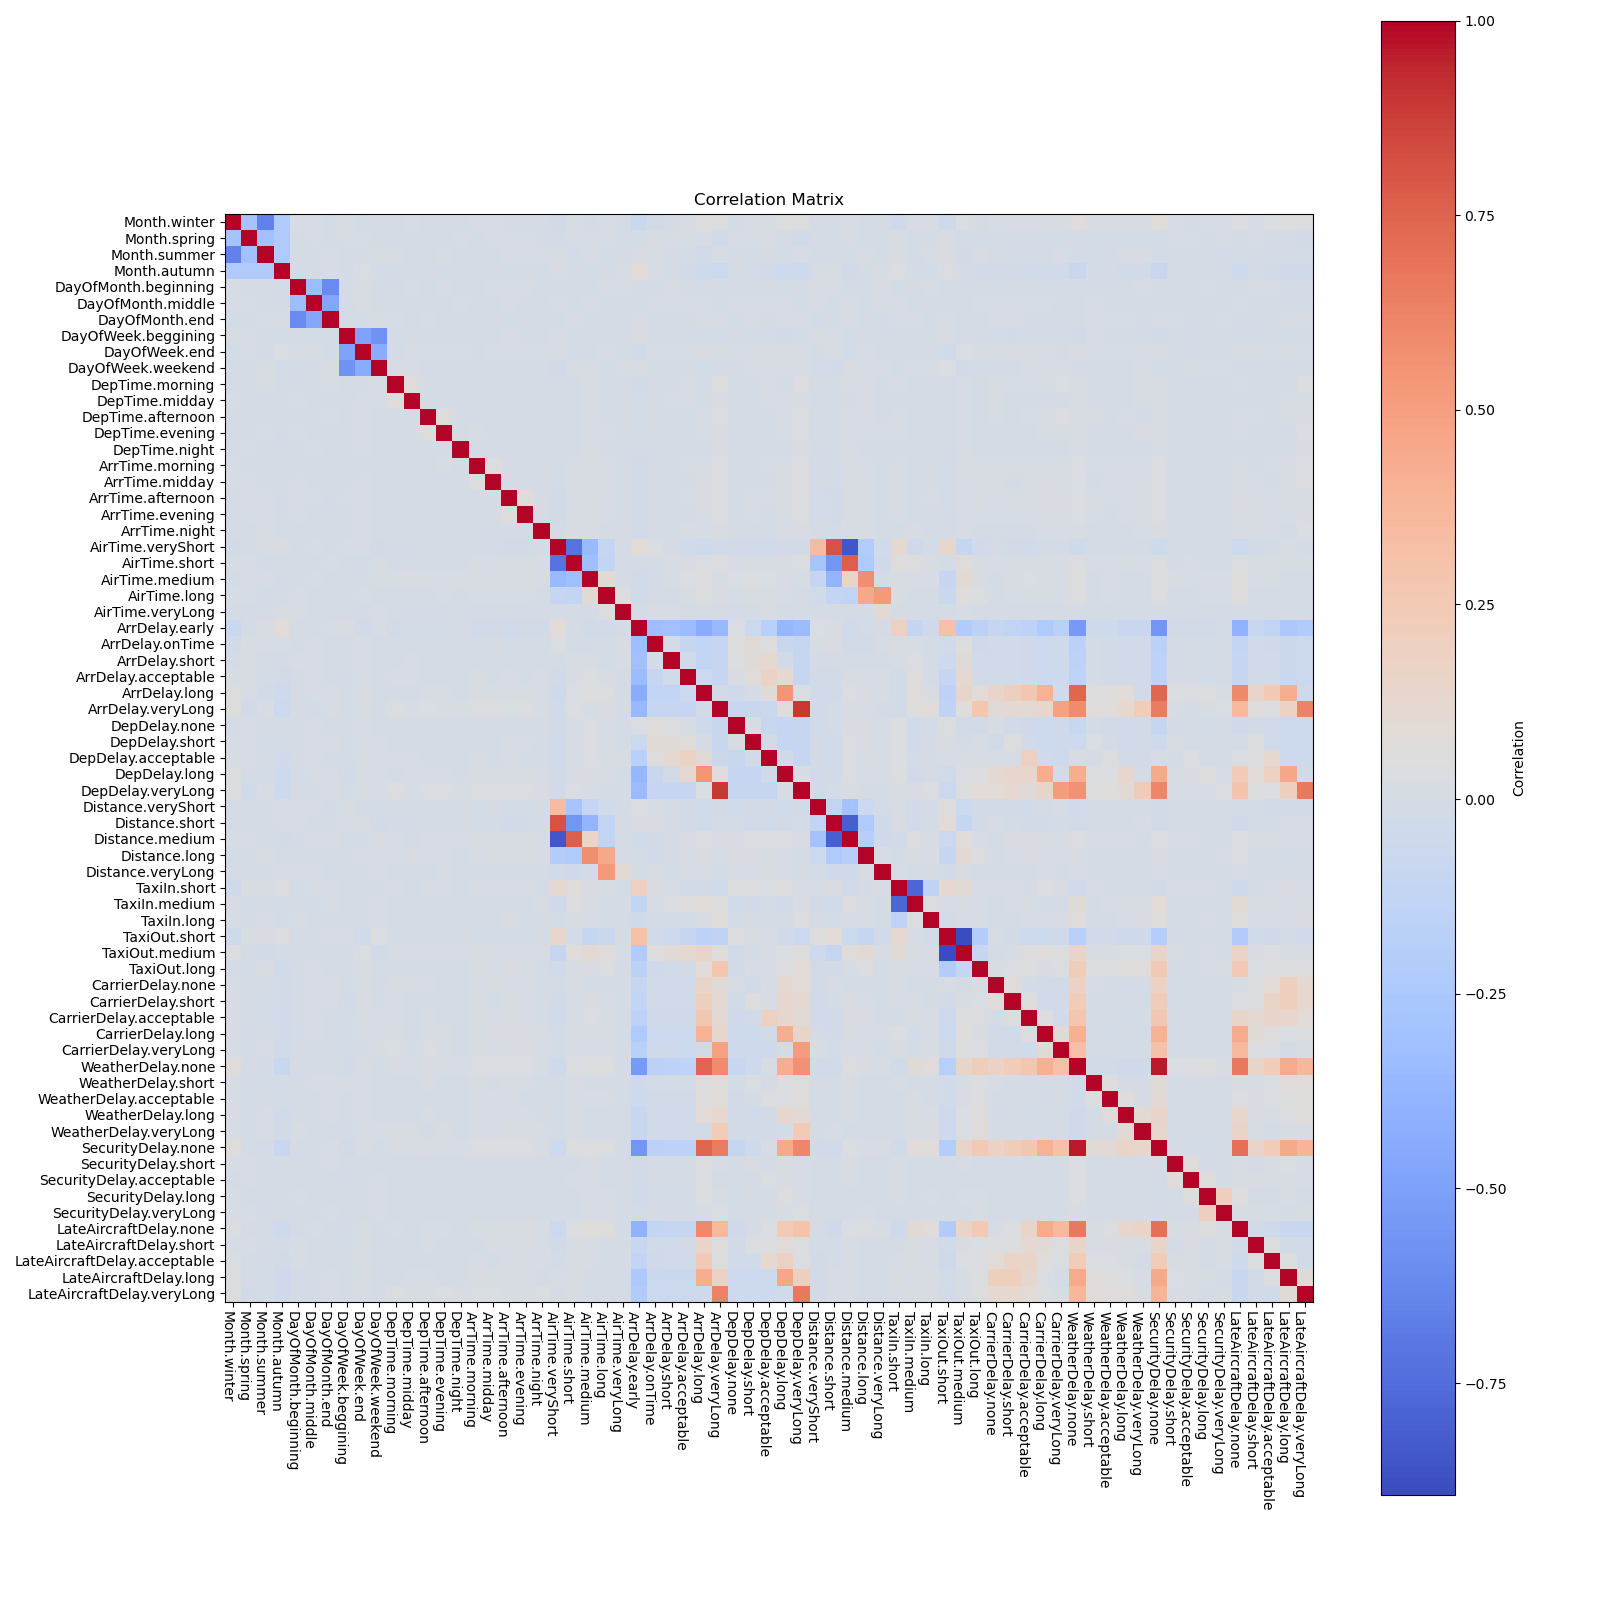
\includegraphics[scale=0.45]{images/correlation_matrix.png}
  \caption{}
  \label{fig:correlation}
\end{figure}

Sur la matrice de corrélation obtenue [fig:\ref{fig:correlation}], nous pouvons encore une fois observée des choses qui étaient attendues, comme le fait que 'AirTime.veryShort' soit positivement corrélé à 'Distance.short' et négativement à 'Distance.medium'.
